\RequirePackage[l2tabu, orthodox]{nag}
\documentclass[]{memoir}

\usepackage{microtype}
\usepackage[dutch]{babel} 
\usepackage{titling}
\usepackage{graphicx}
\usepackage{float}

\graphicspath{{resources/}}
\textwidth=15cm
\setlength{\oddsidemargin}{12pt} 
\setlength{\evensidemargin}{12pt}

%opening
\begin{document}


\begingroup% Scripts, T&H p 151
\centering
\vspace*{0.1\textheight}
{\Huge Het Access Management Systeem}\\[\baselineskip]
{\large\itshape Handleiding}\\[\baselineskip]
\vfill
\rule{0.4\textwidth}{0.4pt}\\[\baselineskip]
{\large\itshape Jeroen De Clerck}\par
\vspace*{0.1\textheight}
\endgroup
\thispagestyle{empty}

\clearpage
\pagenumbering{roman}
\tableofcontents
\clearpage

\pagenumbering{arabic}
%%\chapter{Introductie}
%% wat uitleg over de handleiding zelf, 
%% een verduidelijking van het verschil tussen een Persoon (person), een Partner (Partner) en een Gebruiker (User),
%% een verduidelijking van het verschil tussen een Item en een Material


%% Noot aan schrijver: in de handleiding worden Persoon, Partner en Gebruiker geschreven met hoofdletter als het gaat over een element in de database van het systeem


\chapter{Interface} \label{Interface}
Om de gebruiker wegwijs te maken zullen we eerst in het kort alle elementen van het systeem overlopen. Deze zullen later in detail terugkeren waar nodig. Niet alle opties zijn voor alle gebruikers zichtbaar, dus als er bepaalde elementen onvindbaar zijn, is dat omdat de lezer er niet de correcte rechten voor heeft. Er wordt ten zeerste aangeraden om de onderdelen waar de lezer recht op heeft aandachtig te overlopen voor het lezen van de specifiekere gebruiksaanwijzingen,

\section{Dashboard} \label{Dashboard}
Het centraal overzicht. Bevat een historiek met het aantal personen toegevoegd aan het systeem per dag, plus het aantal verstuurde aanvraagformulieren (\textsl{Submitted Request Forms}) per dag. Dit overzicht kan manueel ververst worden door op het refresh-icoontje te klikken in de rechterbovenhoek. Exacte statistieken van een dag kunnen bekeken worden door met de muis over de grafiek te zweven.

\section{Persons} \label{Persons}
Een overzicht van alle Personen in het systeem. In de tabel kan men de naam, organisatie, categorie, telefoonnummer, aanwezigheid per dag, recht op voorwerpen (\textsl{Items}), laatste aanpassing en status zien. Bij sommige velden is er meer informatie beschikbaar door erover te zweven met de muis. Zo kunnen de meerdere categorien of dagen van een persoon bekeken worden door te zweven over het 'Various' veld in de respectievelijke kolom, of kan het specifieke Voorwerp waar een persoon recht op heeft bekeken worden door te zweven over het Voorwerp-icoontje.\\
Op iedere persoon kan men een aantal acties uitvoeren, namelijk:
\begin{itemize}
	\item Toestaan (\textsl{Approve}), waarmee een persoon toegevoegd via een form toegestaan wordt om in het systeem terecht te komen.
	\item Afwijzen  (\textsl{Deny}), waarmee een persoon toegevoegd via een form afgewezen wordt.
	\item Ticket versturen (\textsl{Send Ticket}), waarmee een mail verstuurd wordt naar het emailadres van de persoon met hun ticket en verdere informatie. Deze optie is enkel zichtbaar nadat de Persoon togestaan werdt.
	\item Aanpassen (\textsl{Edit}), waarmee de Gebruiker naar het profielscherm van de persoon kan gaan, om daar eventueel velden aan te passen.
	\item Verwijderen (\textsl{Delete}), waarmee de persoon uit het systeem verwijderd wordt.
\end{itemize}

Men kan op meerdere personen tegelijk deze acties uitvoeren door ze aan te vinken, en vervolgens in de rechterbovenhoek een optie te selecteren uit het Groepacties  (\textsl{Group Actions}) selectiemenu.\\
Boven de tabel vindt men een filters en een zoekbalk, waarmee respectievelijk alleen de personen aanwezig op de geselecteerde datum getoond worden en respectievelijk met behulp van een tekstveld gezocht kan worden naar specifieke personen. Als laatste zijn er nog twee icoontjes, waarvan de eerste toestaat om een persoon aan te maken op basis van een excel-document, en waarvan het tweede toelaat om manueel een nieuwe persoon toe te voegen aan het systeem.\\


\section{Partners} \label{Partners}
Een overzicht van de Partners ingeschreven in het systeem. Bij het openen ziet de lezer enkel de partners die door hem ingeschreven zijn, maar men kan alle partners zien door linksboven op 'Alle Partners' (\textsl{All Partners}) te klikken. Terugkeren naar het beginscherm kan door op 'Mijn Partners' (\textsl{My Partners}) te klikken.\\
In de partnertabel ziet men de naam van de organisatie, de naam van de verantwoordelijke, of hij al dan niet ingelogd heeft, hoeveel van zijn tickets er verdeeld zijn, \textbf{WAT ZIJN UTILITIES?}, de laatste aanpassing aan de partner, de status en de Gebruiker die deze Partner aangemaakt heeft.\\
Op iedere Partner kan men een aantal acties uitvoeren, namelijk:
\begin{itemize}
	\item Toestaan (\textsl{Approve}), waarmee een Partner toegevoegd via een form  toegestaan wordt om in het systeem terecht te komen.
	\item Afwijzen  (\textsl{Deny}), waarmee een Partner toegevoegd via een form  afgewezen wordt.
	\item ga naar Partner Service Center  (\textsl{Visit PSC}), waarmee de Gebruiker naar het Partner Service Center (PSC) van deze Partner gestuurd wordt. Deze link opent in een nieuw tabblad. Deze optie is enkel zichtbaar nadat de Persoon toegestaan werdt.
	\item verstuur Loginmail  (\textsl{Send Login}), waarmee een mail verstuurd wordt naar het emailadres van Partnerverantwoordelijke met een link naar hun PSC en verdere informatie. Deze optie is enkel zichtbaar nadat de Persoon toegestaan werdt.
	\item Aanpassen (\textsl{Edit}), waarmee de Gebruiker naar het profielscherm van de Partner kan gaan, om daar eventueel velden aan te passen.
	\item Verwijderen (\textsl{Delete}), waarmee de persoon uit het systeem verwijderd wordt.
\end{itemize}
Men kan op meerdere Partners tegelijk deze acties uitvoeren door ze aan te vinken, en vervolgens in de rechterbovenhoek een optie te selecteren uit het Groepacties  (\textsl{Group Actions}) selectiemenu.\\
Als laatste UI-element is er het plus-icoontje rechtsbovenaan de tabel die toestaat om een nieuwe partner aan te maken.

Het is belangrijk om het Partnersysteem niet te verwarren met het Personensysteem. Een Partner is een individu of organisatie, die het recht heeft om een gegeven aantal tickets uit te delen aan collegas. Zo kan bijvoorbeeld een sponser een Partner worden, waardoor de sponser een aantal vip-tickets toegewezen krijgt die uitgedeeld kunnen worden. \textsl{Het uitdelen van deze tickets is dan ook de verantwoordelijkheid van de partner.}

\subsection{Het Partner Service Center} \label{PSC}
Het Partner Service Systeem is dat wat de verantwoordelijke van een Partner te zien krijgt. Het bevat wat informatie over het systeem, contactgegevens van de Gebruiker die de Partner aan het systeem toegevoegd heeft.
De belangrijkste functie van deze pagina is de 'voeg persoon toe'-knop, die een partnerverantwoordelijke toelaat om mensen uit te nodigen. Als de Partner recht heeft op materiaal, is ook de knop 'Alles over voorzieningen' te zien, waarmee de partnerverantwoordelijke specifieke hoeveelheiden van het beschikbare materiaal kan reserveren.

\section{Box Office} \label{Box Office}
\textbf{HOE WERKT DIT?}

\section{Rental} \label{Rental}
Het overzicht voor Materials uit te lenen en terug te nemen. De Gebruiker kan op de grote IN/OUT knoppen klikken om respectievelijk een Material terug te nemen of uit te lenen. \\
\textbf{KUNNEN ENKEL MATERIALS UITGELEEND WORDEN (items hebben een 'rentable' checkbox)?} \\
\textbf{ZO NEE, HOE KUNNEN ITEMS UITGELEEND WORDEN?} \\
\textbf{HOE WERKT FASTSCAN?} \\
\textbf{HOE WERKEN BARCODES VAN PERSONEN?} \\

\section{Reports} \label{Reports}
Geeft een overzicht van:
\begin{itemize}
	\item  hoeveel Personen van welke Categorie er op welke eventdagen toegang hebben.
	\item  hoeveel Items er op welke eventdagen gereserveerd zijn.
\end{itemize}

\section{Configuration} \label{Configuration}
Staat een Gebruiker toe om allerhande instellingen van het syteem aan te passen.
\subsection{Users}
Toont een tabel van Gebruikers, met respectievenlijk hun naam, emailadres, beschikbare UI-elementen en aanmaakdatum. 
Op iedere Gebruiker kan men een aantal acties uitvoeren, namelijk:
\begin{itemize}
	\item Aanpassen (\textsl{Edit}), waarmee men naar het profielscherm van de Gebruiker kan gaan, om daar eventueel velden aan te passen.
	\item Verwijderen (\textsl{Delete}), waarmee de Gebruiker uit het systeem verwijderd wordt.
\end{itemize}
Men kan op meerdere Gebruikers tegelijk deze acties uitvoeren door ze aan te vinken, en vervolgens in de rechterbovenhoek een optie te selecteren uit het Groepacties  (\textsl{Group Actions}) selectiemenu.\\
Verder kan men met behulp van de zoekbalk zoeken naar een specifieke gebruiker, en kan met met behulp van het plus-icoontje in de rechterbovenhoek een nieuwe gebruiker aanmaken.

\subsection{Roles} \label{Roles}
Staat toe om een aantal voorgedefinieerde Rollen aan te maken die specifieke vergunningen in het systeem hebben, en die vervolgens toegewezen kunnen worden aan een Gebruiker.\\
langs de linkerkant staan de geconfigureerde Rollen, en langs de rechterkant kan men een nieuwe Rol aanmaken. 
Specifieke Rollen kunnen verwijderd (\textsl{Delete}) of aangepast (\textsl{Edit}) worden met behulp van het actiemenu (\textsl{Action}).
Men kan meerdere Rollen tegelijk verwijderen door ze aan te vinken, en vervolgens in de rechterbovenhoek 'verwijderen' te selecteren uit het Groepacties  (\textsl{Group Actions}) selectiemenu.\\

\subsection{Categories} \label{Categories}
Staat toe om een aantal voorgedefinieerde Categorien aan te maken die toegewezen kunnen worden aan een Persoon.
In de tabel ziet men een opsomming van de huidige Categorien, met hun naam, de naam die voor deze categorie gebruikt wordt in het Partner Service Centrum, en of al dan niet hun mailtekst, tickettekst en procedure ingevuld zijn in het systeem.
Op iedere Categorie kan men naast Aanpassen (\textsl{Edit}) en Verwijderen (\textsl{Delete}) ook nog een aantal acties uitvoeren, namelijk:
\begin{itemize}
	\item Aanvraagformulier bekijken (\textsl{Visit Request Form}), waarmee de gebruiker het aanvraagformulier voor een ticket van die categorie te zien krijgt. Deze link opent in een nieuw tabblad.
	\item Exporteer (\textsl{Export}), waarmee informatie over de categorie in de vorm van een Excel-bestand gedownload kan worden.
\end{itemize}
Men kan meerdere Categorien tegelijk verwijderen door ze aan te vinken, en vervolgens in de rechterbovenhoek de 'verwijderen'optie te selecteren uit het Groepacties  (\textsl{Group Actions}) selectiemenu.

\subsection{Items \& Materials} \label{ItAndMats}
\subsubsection{Items} \label{Items}
Een overzicht van de Voorwerpen (\textsl{Items}) in het systeem. In de tabel ziet men de naam, onder welke verzamelnaam het voorwerp zich bevindt, of het aan een Persoon of een Partner uitgeleend moet worden, een kolom met icoontjes die extra informatie toont en de aanmaakdatum van het Voorwerp.
De kolom met icoontjes geeft een snel overzicht of een Voorwerp zichtbaar is in het Verslagmenu (\textsl{Reports}), of het een extra ticket nodig heeft, en of het Voorwerp enkel op specifieke dagen beschikbaar is.
\textbf{HOE WERKT DATE DEPENDENCY?}
Specifieke Voorwerpen kunnen verwijderd (\textsl{Delete}) of aangepast (\textsl{Edit}) worden met behulp van het actiemenu (\textsl{Action}).

Onderaan de pagina zijn ook de Voorwerpveld- en Voorwerpgroeptabellen zichtbaar. Dit zijn onderdelen van een Voorwerpbeschrijving en kunnen op dezelfde manier als een Voorwerp aangemaakt, aangepast of verwijderd worden.

\subsubsection{Materials} \label{Materials}
Het is belangrijk om een Voorwerp niet te verwarren met Materiaal. Een Voorwerp heeft een stock, en er kunnen dus 1 of meerdere zelfde Voorwerpen uitgeleend worden aan verschillend Personen of Partners. Een Voorwerp kan uitleenbaar (\textsl{Rentable}) gemaakt worden, waarna ieder apart instantie van dit Voorwerp een barcode moet toegewezen worden in het Materiaalmenu, zodat ze via het Uitleenmenu (\textsl{Rental}) uitgeleend kan worden.

Links op het scherm ziet men een overzicht van alle Materialen in het systeem met hun naam, barcode en Voorwerptype. Men kan deze aanpassen of verwijderen met behulp van het actieselectieveld (\textsl{Action})
Rechts op het scherm kan de Gebruiker materiaal toevoegen door het Voorwerptype te selecteren, de naam in te geven en de barcode te scannen.
\subsection{Zones} \label{Zones}
Links staat een overzicht van alle Zones op het terrein, rechts een klein menuutje waar nieuwe zones mee aangemaak kunen worden. Hier kunnen weer Zones aangemaak of aangepast worden, per stuk of in groep, met behulp van de Actie- en Groepactieknoppen

\subsection{General} \label{General}
Bevat een hoop instellingen met betrekking tot het festival zelf (o.a. tickettemplates, tekstjes voor mails en het Partner Service Systeem). Meer info hierover is te vinden onder Sectie \ref{SetSystem}.

\subsection{Integrations} \label{Integrations}
\textbf{HOE WERKT DIT?}

\subsection{Fields} \label{Fields}
\textbf{HOE WERKT DIT?}

\chapter{Gebruiksaanwijzingen} \label{Instructions}

\section{Admin} \label{AdminInstr}
\subsection{Het systeem instellen.} \label{SetSystem}
Ga naar het Configuratie>Algemeen menu (zie \ref{General}). Hier ziet men de algemene instellingen van het systeem. Ieder veld met een sterretje naast is een veld dat verplicht ingevuld moet worden.
\subsubsection{General}
\subsubsection{Mails}
Hier wordt de ticketmail ingesteld. Men kan hier respectievelijk de naam van de verzender, het adres van de verzender, het onderwerp van de mail, de tekst van de mailm de voetnote voor het onleesbaar zijn van de mail en de voetnote voor een link naar een online versie van de mail aanpassen.
\subsubsection{Tickets}
Hier wordt de achtergrondafbeelding van de printbare tickets ingesteld. De bedoeling is dat men op basis van het gegeven template een nederlandstalige en engelstalige versie van en ticket maakt en deze upload in het systeem. Eens dat deze afbeeldingen zich in het systeem bevinden kunnen ze opnieuw bekeken worden door op bestandsnaam te klikken.
\subsubsection{Wristbands}
\textbf{HOE WERKT DIT?}
\subsubsection{PSC}
\subsection{Een Gebruiker toevoegen} \label{AddUser}
\subsection{Een Rol toevoegen} \label{SetRole}
\subsection{Een Categorie toevoegen} \label{SetCategory}
\subsection{Een Voorwerp toevoegen} \label{SetItem}
Voor een Voorwerp toe te voegen aan het systeem, ga naar het Items (\ref{Items}) menu. \\
\begin{figure}[H]
	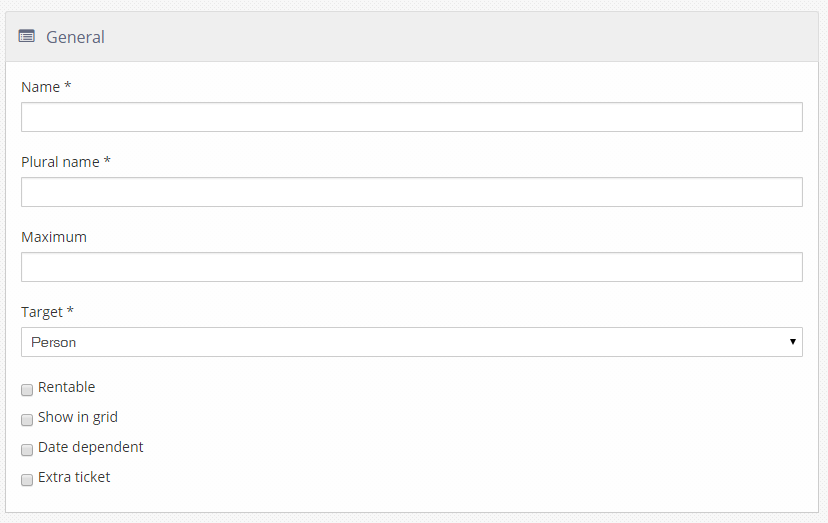
\includegraphics[width=\linewidth]{addItem_left}
	\caption{een Voorwerp aanmaken}
\end{figure}
Vul de naam van een enkelvoudig item en het meervoud van deze naam in.
\textbf{Vervolgens kan men optioneel nog het maximum aantal van dit Voorwerp invullen onder Maximum}, 
Selecteer in het Target selectiemenu of dit item voor Partners of Personen is. \\
Vervolgens zijn er een aantal aantikbare opties.
\begin{itemize}
	\item \textsl{Rentable} zorgt dat dit Voorwerp geindexeerd kan worden als Materiaal en bijgevolg uitgeleend kan worden in het Rentalmenu (\ref{Rental}), 
	\item \textsl{Show in grid} zorgt dat het item zichtbaar is in het Reportsmenu (\ref{Reports}), 
	\item \textsl{Date dependent} betekent dat om het Voorwerp te reserveren, er ook de dagen waarop het gereserveerd wordt geselecteerd moeten worden.
	\item \textsl{Extra Ticket} zorgt dat bij het reserveren van het Voorwerp een extra ticket afgeprint moet worden (denk aan Parkeertickets). Als dit laatste aangevinkt wordt moet er ook een tweetalige tickettekst opgegeven worden.
\end{itemize} 
\begin{figure}[H]
	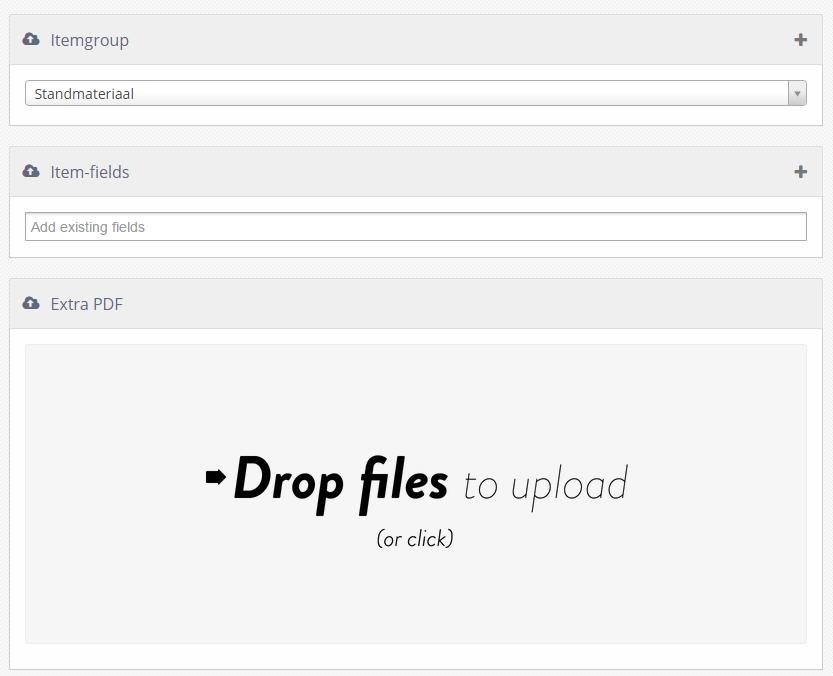
\includegraphics[width=\linewidth]{addItem_right}
	\caption{een Voorwerp aanmaken}
\end{figure}
Selecteer in het itemgroup selectiemenu onder welke itemgroup dit voorwerp valt. 
Voeg onder Item-fields toe welke welk soort beschrijving de partners zullen kunnen of moeten opgeven in het Partner Service Centrum. 
\textbf{Ten laatste kan men een .pdf uploaden om dingen te doen ofzo}
\subsection{Materiaal toevoegen} \label{SetMaterial}
\subsection{Een Zone toevoegen} \label{SetZone}
\subsection{Een Integratie toevoegen} \label{SetIntegration}
\subsection{Een Veld toevoegen} \label{SetField}

\section{Box Office} \label{BoxOfficeInstr}
\subsection{Inchecken} \label{BOCheckIn}
\subsection{Quick Add} \label{BOQuickAdd}

\section{Team Leads} \label{TeamLeadInstr}
\subsection{Een Partner uitnodigen} \label{AddPartner}
Voor een Parter toe te voegen aan het systeem, ga naar het Partners (\ref{Partners}) menu. Linksbovenaan kan u op de plus-knop klikken om naar de aanmaakpagina te gaan.
Op de aanmaakpagina
\subsubsection{Materiaal voor een partner instellen} \label{AddPartnerMaterial}
%%team lead wijst aan welk materiaal een partner mag gebruiken
%%verantwoordelijke kan in het PSC een aanvraag indienen met een aantal voor enkel de toegewezen materialen.

\section{Partners} \label{PartnerInstr}
\subsection{Utilities aanvragen.} \label{RequestMaterial}

\end{document}
